% $Header$

\documentclass[aspectratio=1610]{beamer}

\mode<presentation>
{%
  \usetheme{Boadilla}
}


\usepackage[english]{babel}
\usepackage[utf8]{inputenc}
\usepackage[T1]{fontenc}

\usepackage{%
    animate,
    graphicx,
    varwidth,
    tcolorbox,
    clrscode3e,
    tikz,
    mathtools,
}
\usetikzlibrary{shapes.multipart, trees, overlay-beamer-styles}

\tikzset{%
    block/.style={%
        font=\sffamily,
        draw=black,
        thin,
        fill=pink!50,
        rectangle split,
        rectangle split horizontal,
        rectangle split parts=#1,
        outer sep=0pt
    },
    gblock/.style={%
        block,
        rectangle split parts=#1,
        fill=green!30
    },
    invisible/.style={opacity=0},
    visible on/.style={alt={#1{}{invisible}}},
    alt/.code args={<#1>#2#3}{%
      \alt<#1>{\pgfkeysalso{#2}}{\pgfkeysalso{#3}} % \pgfkeysalso doesn't change the path
    },
    every node/.style={draw, circle, minimum size=.5cm, scale=0.5},
    edge from parent/.style={draw},
    level distance=1cm,
    level 1/.style={sibling distance=5em},
    level 2/.style={sibling distance=2.5em},
    % level 3/.style={sibling distance=1em}
    bchild/.style={draw,thick}, % bold child
}

\graphicspath{{../../imgs/}}

% alert a whole line (especially for algorithms)
\newcommand{\alertline}{%
 \usebeamercolor[fg]{normal text}%
 \only{\usebeamercolor[fg]{alerted text}}}

% floor command
\newcommand{\floor}[1]{\left\lfloor #1 \right\rfloor}

\title[ALG25 - Lecture 5]
{Binary Search Trees}

\subtitle
{Algorithms and Datastructures, F25, Lecture 5}

\author[Andreas H. Høeg-Petersen]
{Andreas Holck Høeg-Petersen}

\institute[AAU]{%
  Department of Computer Science\\
  Aalborg University
}

\date {\today}

\pgfdeclareimage[height=0.5cm]{university-logo}{../../imgs/aau-logo}
\logo{%
    \begin{tikzpicture}[overlay,remember picture]
        \node[left=0.2cm] at (current page.30){\pgfuseimage{university-logo}};
    \end{tikzpicture}
}

\AtBeginSection[]
{%
  \begin{frame}<beamer>{Outline}
    \tableofcontents[currentsection,currentsubsection]
  \end{frame}
}


\begin{document}

\begin{frame}
  \titlepage
\end{frame}

\begin{frame}{Opdateringer}{}
    \begin{itemize}[<+->]
        \small
        \item Næste programmeringsopgave kommer til at handle om binære
            søgetræer (og måske lidt priority queues)
        \item Den skal afleveres i starten af april (nærmere info senere)
        \item Fra evaluering:
            \begin{itemize}
                \item Det `dårlige':
                    \begin{itemize}
                        \item `Meget læsestof til forelæsningen'
                        \item `Flere konkrete eksempler' + `De sidste slides gik
                            lige hurtigt nok' + `ville ønske jeg kunne sætte
                            playback speed x1.25'
                        \item `Svært at se laser nogle gange'
                    \end{itemize}
                \item Det `gode':
                    \begin{itemize}
                        \item `Interessant emne' <3
                        \item `er glad for at du prøver at sørge for alle er
                            med' + `kan godt lide at du spørger ud og er meget
                            opmærksom på os studerende'
                        \item Illustrationer og tegninger på tavlen
                        \item `Hjælpelærer Jakob var vildt god, specielt i
                            første time'
                        \item `opdeling i 2 blokke er en fantastisk formular'
                    \end{itemize}
            \end{itemize}
        \item Næste uge: self-study session med rigtigt eksamenssæt!
    \end{itemize}
\end{frame}


\begin{frame}{Outline}
  \tableofcontents
\end{frame}


\section{Repræsentation af træer}

\begin{frame}{Repræsentation af træer}{Arrays}
    Sidste gang så vi på \alert{binære heaps}, hvor vi fortolkede et array
    $A[1:n]$ som et binært træ.

    \pause

    \begin{figure}[h]
        \centering
        \includegraphics[width=0.4\textwidth]{heaps/array}
        \includegraphics[width=0.4\textwidth]{heaps/tree}
    \end{figure}

    \pause

    I dette tilfælde antager vi, at træet er \alert{næsten komplet}, og at et
    element $A[i]$ er forældreknude til elementerne $A[2i]$ og $A[2i + 1]$ (så
    længe $2i \leq n$ og $2i + 1 \leq n$).
\end{frame}


\begin{frame}{Repræsentation af træer}{Begrænsninger for arrays}
    Hvilke begrænsninger giver dette os?

    \begin{itemize}[<+->]
        \item<2-> Træet \alert{skal} fyldes op fra `venstre mod højre'
        \item<3-> Træets størrelse er begrænset til $n$ (og skal være kendt på
            forhånd)
        \item<4-> Hver knude kan kun have 2 børn (eller skal i hvert fald have
            det samme antal børn)
    \end{itemize}

    \uncover<5->{En mere generisk løsning? \alert{Pointers}!}
\end{frame}


\begin{frame}{Repræsentation af træer}{Generalisering med pointers}
    Når vi repræsenterer et binært træ $T$ med pointers, så gør vi følgende:

    \begin{columns}
        \column{.5\textwidth}
        \begin{itemize}[<+(1)->]
            \item Hver knude $x$ i træet er et objekt med 4 attributter:
                \begin{itemize}
                    \item $\attrib{x}{key}$ indeholder knudens værdi/nøgle
                    \item $\attrib{x}{p}$ peger på knudes forældre (\alert{parent})
                    \item $\attrib{x}{left}$ og $\attrib{x}{right}$ peger hhv.\ på
                        knudens venstre og højre barn
                \end{itemize}
            \item $\attrib{T}{root}$ peger på træets rod --- bemærk at
                $\attrib{x}{p} = \const{NIL}$ hvis og kun hvis $x =
                \attrib{T}{root}$
        \end{itemize}    

        \uncover<+(1)->{Nu kan vi nemt indsætte nye knuder, hvor vi vil (bare
        opdater pointers) og træet kan gro til en arbitrær størrelse.}

        \column{.5\textwidth}
        \begin{figure}[h]
            \centering
            \includegraphics[width=0.8\textwidth]{rooted-binary-tree}
        \end{figure}

    \end{columns}
    
\end{frame}


\begin{frame}{Repræsentation af træer}{Bonus: ubegrænset forgrening}
    I vores repræsentation af et træ kan hver knude stadig kun have 2 børn. Kan
    vi løse det?

    \pause
    \begin{itemize}[<+->]
        \item Vi kunne give hver knude $k$ børn, som vi kan tilgå med
            $\attrib{x}{child_1}, \attrib{x}{child_2}, \ldots,
            \attrib{x}{child_k}$
            \begin{itemize}
                \item Men så er vi tilbage til, at alle knuder \alert{maksimalt}
                    kan have $k$ børn og\ldots
                \item at vi \alert{skal} sætte plads af til $k$ børn i alle
                    knuder, uanset at de fleste knuder måske har meget færre
            \end{itemize}
        \item En bedre løsning med ubegrænset forgrening kaldes
            \alert{left-child, right-sibling} repræsentationen
            \begin{itemize}
                \item Vi erstatter $\attrib{x}{left}$ og $\attrib{x}{right}$ med
                    \begin{itemize}
                        \item $\attrib{x}{left-child}$, der peger på knudens
                            barn længst til venstre
                        \item $\attrib{x}{right-sibling}$, der peger på knudens
                            søskende umiddelbart til højre
                    \end{itemize}
                \item Søskende-relationen bliver dermed en slags \alert{linked
                    list} repræsentation, der tillader forskelligt antal børn
                    for hver enkelt knude
            \end{itemize}
    \end{itemize}
\end{frame}


\begin{frame}{Repræsentation af træer}{Left-child, right-sibling}
    \begin{figure}[h]
        \centering
        \includegraphics[width=0.8\textwidth]{left-child-right-sib-tree}
    \end{figure}
\end{frame}

\begin{frame}{Repræsentation af træer}{Back to basics}
    \centering
    Men da vi nu udelukkende skal se på \alert{binære træer}, så holder vi os
    til den simple repræsentation med $\attrib{x}{left}$ og
    $\attrib{x}{right}$\ldots
\end{frame}

\section{Binære søgetræer}

\begin{frame}{Binære søgetræer}{Hvad og hvorfor}
    En klassisk og udbredt datastruktur er de binære søgetræer eller
    \alert{binary search trees} eller bare BST'er. 

    \begin{itemize}
        \item Understøtter operationer som $\proc{Insert}$, $\proc{Search}$,
            $\proc{Delete}$, $\proc{Minimum}$ og $\proc{Maximum}$
        \item De kan således bruges som
            \begin{itemize}
                \item \alert{dictionaries}, der associerer en nøgle
                    (\alert{key}) til en værdi (\alert{value})
                \item \alert{priority queues}, der opretholder en orden på basis
                    af nøgler
            \end{itemize}
        \item Operationer på BST'er er proportionelle til træets højde $h$
            \begin{itemize}
                \item For et balanceret træ med $n$ knuder er højden $O(\log n)$
                \item I worst-case er træet dog så ubalanceret, at højden er
                    $O(n)$
            \end{itemize}
    \end{itemize}
\end{frame}

\begin{frame}{Binære søgetræer}{BST-egenskaben}
    Ligesom vi havde en heap-egenskab, som alle knuder i et heap skulle
    overholde, så har vi også en egenskab for BST'er:

    \pause
    \begin{block}{Binary-search-tree property}
        For to knuder $x, y$ i et binært søgetræ:

        \begin{itemize}
            \item Hvis $y$ er en knude i det venstre sub-træ af $x$, så skal
                $\attrib{y}{key} \leq \attrib{x}{key}$ 
            \item Hvis $y$ er en knude i det højre sub-træ af $x$, så skal
                $\attrib{y}{key} \geq \attrib{x}{key}$ 
        \end{itemize}
    \end{block}

    \pause
    Hvordan adskiller det sig fra et heap?

    \pause
    \begin{block}{Max-Heap property}
        For alle knuder $i > 1$ gælder $A[\proc{Parent}(i)] \geq A[i]$
    \end{block}
\end{frame}

\begin{frame}{Binære søgetræer}{BST-egenskaben}
    Mere uformelt siger vi, at alt til venstre skal være \alert{mindre end}
    eller lig med, og at alt til højre skal være \alert{større end} eller lig
    med. \\

    \pause
    Er disse træer BST'er?

    \vfill
    \begin{columns}
        \column{.24\textwidth}
        \centering
        \pause
        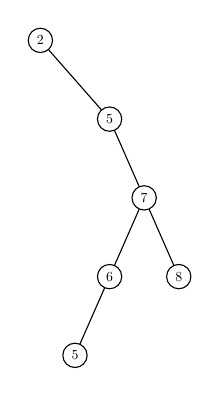
\begin{tikzpicture}
            \node {2}
                child[missing]{}
                child {node {5}
                    child[missing]{}
                    child {node {7}
                        child {node {6}
                                child {node {5} }
                                child[missing]{}
                            }
                        child {node{8} }
                    }
                };
        \end{tikzpicture}

        \pause
        Ja!
    
        \column{.24\textwidth}
        \centering

        \pause

        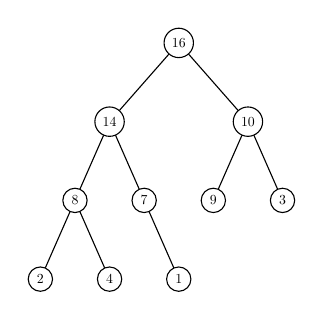
\begin{tikzpicture}
            \node {16}
                child {node {14}
                    child {node {8}
                        child {node {2}}
                        child {node {4}}
                    }
                    child {node {7}
                        child[missing]{}
                        child {node {1}}
                    }
                }
                child {node {10}
                    child {node {9}}
                    child {node {3}}
                };
        \end{tikzpicture}

        \pause
        Nej!

        \column{.24\textwidth}
        \centering

        \pause

        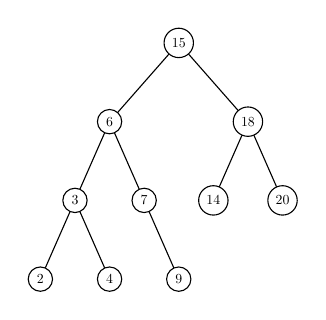
\begin{tikzpicture}
            \node {15}
                child {node {6}
                    child {node {3}
                        child {node {2}}
                        child {node {4}}
                    }
                    child {node {7}
                        child[missing]{}
                        child {node{9}}
                    }
                }
                child {node {18}
                    child {node {14}}
                    child {node {20}}
                };
        \end{tikzpicture}

        \pause
        Nej!

        \column{.24\textwidth}
        \centering

        \pause

        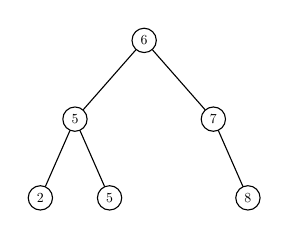
\begin{tikzpicture}
            \node {6}
                child {node {5}
                    child {node {2}}
                    child {node {5}}
                }
                child {node {7}
                    child[missing]{}
                    child {node {8}}
                };
        \end{tikzpicture}

        \pause
        Ja!
    \end{columns}
\end{frame}


\begin{frame}{Binære søgetræer}{Traversere træet}
    Vi ser senere på, hvordan vi indsætter og sletter fra et BST.\ Først, hvad
    kan vi med et BST?

    \begin{columns}
        \column{.5\textwidth}
        \begin{itemize}
            \item<1-> Vi kan udnytte BST-egenskaben til at printe alle nøglerne i
                sorteret rækkefølge
            \item<2-> $\proc{Inorder-Tree-Walk}(x)$ tager en knude $x$ og
                printer først alle nøgler i det venstre (lille) sub-træ, så
                $\attrib{x}{key}$ og til sidst alle nøgler i det højre (store)
                sub-træ
            \item<3-> Kompleksitet? \uncover<4->{$\Theta(n)$ (for et træ med $n$
                knuder)}
        \end{itemize}
    
        \column{.5\textwidth}
        \begin{block}{$\proc{Inorder-Tree-Walk}(x)$}
            \small

            \vspace{-\abovedisplayskip}
            \begin{codebox}
                \li \If $x \neq \const{NIL}$
                \li \Then
                        $\proc{Inorder-Tree-Walk}(\attrib{x}{left})$
                \li     print $\attrib{x}{key}$ 
                \li     $\proc{Inorder-Tree-Walk}(\attrib{x}{right})$
                    \End
            \end{codebox}
        \end{block}
        \centering
        \vfill
        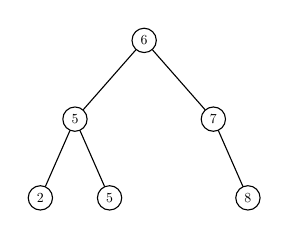
\begin{tikzpicture}
            \node {6}
                child {node {5}
                    child {node {2}}
                    child {node {5}}
                }
                child {node {7}
                    child[missing]{}
                    child {node {8}}
                };
        \end{tikzpicture}
    \end{columns}
\end{frame}


\begin{frame}{Søgning}{}
    For søgning i træet har vi følgende simple procedure:

    \begin{columns}
        \column{.5\textwidth}
        \begin{block}{$\proc{Iterative-Tree-Search}(T,k)$}
            \small
            
            \vspace{-\abovedisplayskip}
            \begin{codebox}
                \li \While $x \neq \const{NIL}$ and $\attrib{x}{key} \neq k$
                    \Do
                    \li \If $k < \attrib{x}{key}$
                        \Then
                            \li $x = \attrib{x}{left}$ 
                        \li \Else 
                            $x \gets \attrib{x}{right}$ 
                        \End
                    \End
                \li \Return $x$
            \end{codebox}
        \end{block}

        \begin{figure}[h]
            \centering
            \includegraphics[width=0.6\textwidth]{bst/tree-search}
        \end{figure}
    
        \column{.5\textwidth}
        \begin{itemize}
            \small
            \item<2-> While-løkken tester, om $x$ er $\const{NIL}$ (søgningen har
                fejlet) eller $\attrib{x}{key} = k$ (søgningen er successfuld)
            \item<3-> Hvis $k$ er mindre end $\attrib{x}{key}$ skal vi lede videre i
                det venstre sub-træ (vi sætter $x = \attrib{x}{left})$ --- og
                ellers skal vi lede i det højre sub-træ
            \item<4-> Vi slutter, når vi enten har fundet det rigtige element eller
                $x$ er sat til $\const{NIL}$
            \item<5-> Kompleksitet?
                \begin{itemize}
                    \item<6-> Hver iteration bevæger sig et niveau ned i træet
                    \item<7-> Der er maks $h$ niveauer, så kompleksiteten er
                        $O(h)$
                \end{itemize}
            \item<8-> En rekursiv udgave findes også, men den vil typisk være
                mindre effektiv
        \end{itemize}
    \end{columns}
\end{frame}


\begin{frame}{Minimum og Maximum}{}
    Vi har også to simple procedurer til at finde det største og mindste element
    i et træ.

    \begin{columns}
        \column{.6\textwidth}
        \begin{itemize}[<+(1)->]
            \small
            \item $\proc{Tree-Minimum}(x)$ følger blot stien, der fremkommer ved
                at fortsætte til venstre i træet indtil, at den når et blad
            \item $\proc{Tree-Maximum}(x)$ gør det samme, denne gang bare ved at
                gå mod højre
            \item BST-egenskaben garanterer korrektheden af disse metoder
            \item Begge kører i $O(h)$
        \end{itemize}

        \begin{figure}[h]
            \centering
            \includegraphics[width=0.4\textwidth]{bst/tree-min-max}
        \end{figure}
    
        \column{.4\textwidth}
        \small
        \begin{block}{$\proc{Tree-Minimum}(x)$}
            
            \vspace{-\abovedisplayskip}
            \begin{codebox}
                \li \While $\attrib{x}{left}\neq \const{NIL}$ \Do
                \li $x \gets \attrib{x}{left}$ 
                \End
                \li \Return $x$
            \end{codebox}
        \end{block}
        \vfill
        \begin{block}{$\proc{Tree-Maximum}(x)$}
            
            \vspace{-\abovedisplayskip}
            \begin{codebox}
                \li \While $\attrib{x}{right}\neq \const{NIL}$ \Do
                \li $x \gets \attrib{x}{right}$ 
                \End
                \li \Return $x$
            \end{codebox}
        \end{block}
    \end{columns}
\end{frame}


\begin{frame}{Predecessor og successor}{}
    De to foregående procedurer kan vi blandt andet benytte til at konstruere
    procedurer for at finde en knudes \alert{predecessor} og \alert{successor}.

    \begin{columns}
        \column{.5\textwidth}
        \begin{itemize}
            \item Givet en knude $x$ i et BST $T$ returnerer
                $\proc{Tree-Successor}$ den knude, som har den \alert{mindste}
                nøgle, der er \alert{større} end $\attrib{x}{key}$
            \item<2-> Der er to cases:
                \begin{itemize}
                    \item<3-> 1) Enten er successoren det mindste element i det
                        højre (altså store) sub-træ til $x$
                    \item<4-> 2) Ellers skal vi kravle op i træet indtil, at vi
                        finder den første knude, som har $x$ i sit venstre
                        (lille sub-træ)
                \end{itemize}
            \item<5-> Der er en helt analog procedure for at finde predecessor
                (største element, der er mindre end $x$)
        \end{itemize}
    
        \column{.5\textwidth}
        \begin{block}{$\proc{Tree-Successor}(x)$}
        
            \vspace{-\abovedisplayskip}
            \begin{codebox}
                \li \alertline<3>\If $\attrib{x}{right} \neq \const{NIL}$
                \li \alertline<3>\Then
                        \alertline<3>\Return $\proc{Tree-Minimum}(\attrib{x}{right})$
                \li \Else
                \li     \alertline<4>$y \gets \attrib{x}{p}$
                \li     \alertline<4>\While $y \neq \const{NIL}$ and $x \isequal \attrib{y}{right}$ 
                            \Do
                \li             \alertline<4>$x \gets y$
                \li             \alertline<4>$y \gets \attrib{y}{p}$ 
                            \End
                    \End
                \li \alertline<4>\Return $y$
            \end{codebox}
        \end{block}

    \end{columns}
\end{frame}


\begin{frame}{Successor}{Eksempel}
    \begin{columns}
        \column<2->{.31\textwidth}
        \centering

        $\proc{Tree-Successor(15)}$
    
        \column<3->{.31\textwidth}
        \centering

        $\proc{Tree-Successor}(13)$

        \column{.36\textwidth}
    \end{columns}

    \begin{columns}
        \column<2->{.31\textwidth}
        \begin{figure}[h]
            \centering
            \includegraphics[width=0.9\textwidth]{bst/tree-successor-15}
        \end{figure}
    
        \column<3->{.31\textwidth}
        \begin{figure}[h]
            \centering
            \includegraphics[width=0.9\textwidth]{bst/tree-successor-13}
        \end{figure}

        \column{.36\textwidth}
        \begin{block}{$\proc{Tree-Successor}(x)$}
            \scriptsize
        
            \vspace{-\abovedisplayskip}
            \begin{codebox}
                \li \If $\attrib{x}{right} \neq \const{NIL}$
                \li \Then
                        \Return $\proc{Tree-Minimum}(\attrib{x}{right})$
                \li \Else
                \li     $y \gets \attrib{x}{p}$
                \li     \While $y \neq \const{NIL}$ and $x \isequal \attrib{y}{right}$ 
                            \Do
                \li             $x \gets y$
                \li             $y \gets \attrib{y}{p}$ 
                            \End
                    \End
                \li \Return $y$
            \end{codebox}
        \end{block}
    \end{columns}

    \begin{columns}[t]
        \column<2->{.31\textwidth}
        \small

        Successoren til knuden med nøgle 15 er det mindste element i det højre
        sub-træ.
    
        \column<3->{.31\textwidth}
        \small

        Knuden med nøgle 13 har ikke noget sub-træ til højre, så dens successor
        er den mindste ancestor (`bedsteforældre'), hvis venstre barn også er en
        ancestor til 13.

        \column<4->{.36\textwidth}
        \vfill
        \small
        Kompleksitet?

        \begin{itemize}
        \small
            \item<5-> $\proc{Tree-Minimum}$ kører i $O(h)$
            \item<6-> Linie 3-8\ldots \uncover<7->{traverserer træet og
                kører dermed også i $O(h)$}
        \end{itemize}
    \end{columns}

\end{frame}


\section{Exercises}

\begin{frame}{Exercises}{Super fedt! <3}

    På Moodle! Go! Fungerer det fint?

    \begin{figure}[h]
        \centering
        \includegraphics[width=0.8\textwidth]{exercises}
    \end{figure}
    
\end{frame}

\begin{frame}{Kuriosum}{ChatGPT snyder dig nemt}
    Kan I huske det gode spørgsmål fra 2.\ forelæsning?
    \vfill

    \pause
    \begin{quote}
        Er der et eksempel på en algoritme, hvor der er forskel på upper og
        lower bound i worst case?
    \end{quote}

    \vfill
    \pause
    Lad os spørge ChatGPT!
\end{frame}



\begin{frame}{Binære søgetræer}{Hvad har vi set so far?}
    Lad os lige samle op:

    \begin{itemize}[<+(1)->]
        \item $\proc{Inorder-Tree-Walk}(x)$ printer alle elementer i træet med
            rod i $x$ ud i sorteret rækkefølge
        \item $\proc{Tree-Search}(T,k)$ returnerer det element, der har nøglen $k$
            (eller $\const{NIL}$, hvis det ikke findes)
        \item $\proc{Tree-Minimum}(x)$ returnerer det mindste element i træet
            med rod i $x$ (og $\proc{Tree-Maximum}(x)$ returnerer omvendt det
            største element)
        \item $\proc{Tree-Successor}(x)$ returnerer det mindste element, der er
            større end $x$
        \item Udover $\proc{Inorder-Tree-Walk}$, som kører i $\Theta(n)$ kører
            alle procedurerne i $O(h)$, hvor $h$ er træets højde
        \item Alt dette lader sig kun gøre pga BST-egenskaben, der siger,at alle
            elementer til venstre for $x$ skal være mindre end $x$ og alle
            elementer til højre skal være større end $x$
    \end{itemize}
    \vfill
    \pause
    Vi ser nu på, hvordan vi kan indsætte og slette fra BST'er, så vi fortsat
    opretholder BST-egenskaben.
\end{frame}

\section{Manipulering med BST'er}

\begin{frame}{Manipulering med BST'er}{Insertion}
    At indsætte i et BST er relativt simpelt.

    \begin{columns}
        \column{.6\textwidth}
        \small

        \begin{itemize}[<+->]
            \item Proceduren tager et træ $T$ og en knude $z$, som vi vil
                indsætte \alert{som et nyt blad i træet}
            \item Vi definerer $x$  til at være den knude, vi sammenligner med
                $z$ (til at starte med $\attrib{T}{root}$), og $y$ er bare
                forældren til $x$
            \item Sålænge $x$ ikke er $\const{NIL}$ sammenligner vi
                $\attrib{z}{key}$ med $\attrib{x}{key}$, og går enten til højre
                eller venstre i træet
            \item Når $x$ er $\const{NIL}$, sætter vi $z$'s parent til at være
                $y$
            \item Hvis $y$ er $\const{NIL}$, er træet tomt, og $z$ skal være den
                nye rod --- ellers indsætter vi $x$ som enten det venstre eller
                højre barn af $y$
        \end{itemize}
    
        \column{.4\textwidth}
        \begin{block}{$\proc{Tree-Insert}(T,z)$}
            \small
        
            \vspace{-\abovedisplayskip}
            \begin{codebox}
                \li \alertline<2>$x \gets \attrib{T}{root}$ 
                \li \alertline<2>$y \gets \const{NIL}$ 
                \li \alertline<3>\While $x \neq \const{NIL}$  
                    \Do
                \li     \alertline<3>$y \gets x$ 
                \li     \alertline<3>\If  $\attrib{z}{key} < \attrib{x}{key}$ 
                        \Then
                \li         \alertline<3>$x \gets \attrib{x}{left}$
                \li     \Else \alertline<3>$x \gets \attrib{x}{right}$
                        \End
                    \End

                \li \alertline<4>$\attrib{z}{p} \gets y$ 

                \li \alertline<5>\If $y \isequal \const{NIL}$ 
                    \Then
                \li \alertline<5>    $\attrib{T}{root} \gets z$ 
                \li \ElseIf \alertline<5>$\attrib{z}{key} < \attrib{y}{key}$ 
                    \Then
                \li \alertline<5>    $\attrib{y}{left} \gets z$
                \li \Else \alertline<5>$\attrib{y}{right} \gets z$
                    \End
            \end{codebox}
        \end{block}
    \end{columns}
\end{frame}


\begin{frame}{Manipulering af BST'er}{Insertion eksempel}
    Lad os prøve at indsætte nøglerne $\langle 12,18,5,2,15,9,17,19,13 \rangle$:

    \begin{columns}
        \column{.3\textwidth}
        \small
        \begin{itemize}[<+(1)->]
            \item $\proc{Tree-Insert}(T,12)$ --- kommer ind som rod
            \item $\proc{Tree-Insert}(T,18)$
            \item $\proc{Tree-Insert}(T,5)$
            \item $\proc{Tree-Insert}(T,2)$
            \item $\proc{Tree-Insert}(T,15)$
            \item $\proc{Tree-Insert}(T,9)$
            \item $\proc{Tree-Insert}(T,17)$
            \item $\proc{Tree-Insert}(T,19)$
            \item $\proc{Tree-Insert}(T,13)$
        \end{itemize}
    
        \column{.3\textwidth}
        \centering
        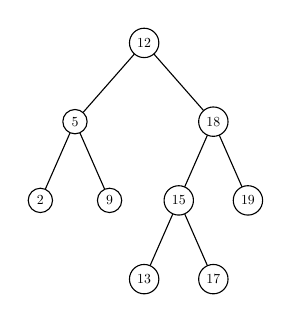
\begin{tikzpicture}
            \node[visible on= <2->] {12}
                child[visible on= <4->] {node{5}
                    child[visible on= <5->] {node{2}}
                    child[visible on= <7->] {node{9}}
                }
                child[visible on= <3->] {node{18}
                    child[visible on= <6->] {node{15}
                        child[visible on= <10->] {node {13}}
                        child[visible on= <8->] {node {17}}
                    }
                    child[visible on= <9->] {node {19}}
                };
        \end{tikzpicture}

        \column{.39\textwidth}
        \begin{block}{$\proc{Tree-Insert}(T,z)$}
            \small
        
            \vspace{-\abovedisplayskip}
            \begin{codebox}
                \li $x \gets \attrib{T}{root}$ 
                \li $y \gets \const{NIL}$ 
                \li \While $x \neq \const{NIL}$  
                    \Do
                \li     $y \gets x$ 
                \li     \If  $\attrib{z}{key} < \attrib{x}{key}$ 
                        \Then
                \li         $x \gets \attrib{x}{left}$
                \li     \Else $x \gets \attrib{x}{right}$
                        \End
                    \End

                \li $\attrib{z}{p} \gets y$ 

                \li \If $y \isequal \const{NIL}$ 
                    \Then
                \li     $\attrib{T}{root} \gets z$ 
                \li \ElseIf $\attrib{z}{key} < \attrib{y}{key}$ 
                    \Then
                \li     $\attrib{y}{left} \gets z$
                \li \Else $\attrib{y}{right} \gets z$
                    \End
            \end{codebox}
        \end{block}
        
    \end{columns}

\end{frame}

\begin{frame}{Manipulering af BST'er}{Insertion worst case}
    Men vent\ldots Hvad nu, hvis vi havde indsat elementerne i sorteret
    rækkefølge?

    \begin{columns}
        \column{.3\textwidth}
        \small
        \begin{itemize}[<+(1)->]
            \item $\proc{Tree-Insert}(T,2)$
            \item $\proc{Tree-Insert}(T,5)$
            \item $\proc{Tree-Insert}(T,9)$
            \item $\proc{Tree-Insert}(T,12)$
            \item $\proc{Tree-Insert}(T,13)$
            \item $\proc{Tree-Insert}(T,15)$
            \item $\proc{Tree-Insert}(T,17)$
            \item $\proc{Tree-Insert}(T,18)$ \alert{NOOOOOOOOO\ldots}
            \item $\proc{Tree-Insert}(T,19)$ \alert{\ldots OOOOOOO!!}
        \end{itemize}
    
        \column{.3\textwidth}
        \centering
        \begin{tikzpicture}
            \node[visible on= <2->] {2}
                child[missing]{}
                child[visible on= <3->] {node{5}
                    child[missing]{}
                    child[visible on= <4->] {node{9}
                        child[missing]{}
                        child[visible on= <5->] {node{12}
                            child[missing]{}
                            child[visible on= <6->] {node{13}
                                child[missing]{}
                                child[visible on= <7->] {node{15}
                                    child[missing]{}
                                    child[visible on= <8->] {node{17}
                                        child[missing]{}
                                        child[visible on= <9->] {node{18}
                                            child[missing]{}
                                            child[visible on= <10->] {node{19}}
                                        }
                                    }
                                }
                            }
                        }
                    }
                };
        \end{tikzpicture}

        \column{.39\textwidth}
        \begin{block}{$\proc{Tree-Insert}(T,z)$}
            \small
        
            \vspace{-\abovedisplayskip}
            \begin{codebox}
                \li $x \gets \attrib{T}{root}$ 
                \li $y \gets \const{NIL}$ 
                \li \While $x \neq \const{NIL}$  
                    \Do
                \li     $y \gets x$ 
                \li     \If  $\attrib{z}{key} < \attrib{x}{key}$ 
                        \Then
                \li         $x \gets \attrib{x}{left}$
                \li     \Else $x \gets \attrib{x}{right}$
                        \End
                    \End

                \li $\attrib{z}{p} \gets y$ 

                \li \If $y \isequal \const{NIL}$ 
                    \Then
                \li     $\attrib{T}{root} \gets z$ 
                \li \ElseIf $\attrib{z}{key} < \attrib{y}{key}$ 
                    \Then
                \li     $\attrib{y}{left} \gets z$
                \li \Else $\attrib{y}{right} \gets z$
                    \End
            \end{codebox}
        \end{block}
        
    \end{columns}
\end{frame}


\begin{frame}{Manipulering af BST'er}{Insertion worst case}
    Med andre ord --- hvis vores data kommer uhensigtsmæssigt ind (f.eks.\
    sorteret), så bliver højden på vores træ $n$, og så har vi basically bare en
    linked liste.
    
    \vfill

    \pause
    Dermed bliver alle vores tidligere operationer også $O(n)$.

    \vfill

    \pause
    Det kan heldigvis vises, at hvis data kommer ind i tilfældig rækkefølge, så
    er den forventede højde på træet $O(\log n)$.

    \vfill

    \pause
    Og næste gang ser vi på en modifikation af BST'er, der garanterer, at træet
    er balanceret.
\end{frame}


\begin{frame}{Manipulering af BST'er}{Deletion}
    Hvor insertion er en relativt simpel procedure, så kræver deletion lidt
    flere tricks. Lad os sige, at vi vil slette en knude $z$:

    \begin{columns}
        \column{.5\textwidth}
        \small
        \begin{itemize}[<+(1)->]
            \item Det er simpelt nok, hvis $z$ er et blad --- så sletter vi den bare
            \item Hvis $z$ kun har 1 barn, så er det også nemt --- så flytter vi
                bare barnet op på $z$'s plads
            \item Men hvis $z$ har 2 børn, så skal vi ind med en skalpel og rode
                lidt
        \end{itemize}    
    
        \column{.5\textwidth}

        \begin{columns}
            \column{.4\textwidth}
            \centering

            % delete leaf
            \only<2>{%
                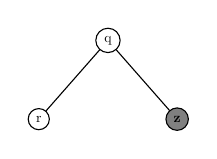
\begin{tikzpicture}[visible on=<2>]
                    \node {q}
                        child {node{r}}
                        child {node[fill=gray]{\textbf{z}}};
                \end{tikzpicture}
            }
        
            % delete node with one child
            \only<3>{%
                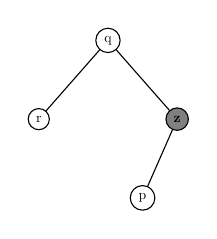
\begin{tikzpicture}
                    \node {q}
                        child {node{r}}
                        child {node[fill=gray]{\textbf{z}}
                            child {node{p}}
                            child[missing]{}
                        };
                \end{tikzpicture}
            }
        
            \only<4>{%
                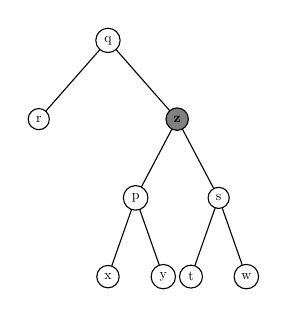
\begin{tikzpicture}[
                    level 2/.style={sibling distance=3em},
                    level 3/.style={sibling distance=2em},
                    ]
                    \node {q}
                        child {node{r}}
                        child {node[fill=gray]{\textbf{z}}
                            child {node{p}
                                child {node{x}}
                                child {node{y}}
                            }
                            child {node{s}
                                child {node{t}}
                                child {node{w}}
                            }
                        };
                \end{tikzpicture}
            }
        
            \column{.2\textwidth}
            \only<2->{$\longrightarrow$}


            \column{.4\textwidth}
            \centering

            % delete leaf
            \only<2>{%
                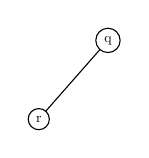
\begin{tikzpicture}
                    \node {q}
                        child {node{r}}
                        child[missing]{};
                \end{tikzpicture}
            }
        
            % delete node with one child
            \only<3>{%
                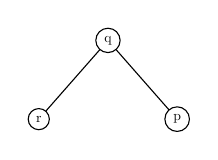
\begin{tikzpicture}
                    \node {q}
                        child {node{r}}
                        child {node{p}};
                \end{tikzpicture}
            }

            \only<4>{%
                \begin{figure}[h]
                    \centering
                    \includegraphics[width=0.7\textwidth]{scalpel}
                \end{figure}
            }
        
        \end{columns}
    \end{columns}

\end{frame}


\begin{frame}{Manipulering af BST'er}{Deletion når der er 2 børn}
    Vi kigger nu på, hvordan vi sletter en knude $z$, når den har 2 børn
    (drabeligt!)

    \begin{columns}
        \column{.5\textwidth}
        \small
        \begin{itemize}[<+(1)->]
            \item Først skal vi finde $z$'s successor $y$. Vi ved, at $y$ ligger i
                $z$'s højre sub-træ og ikke har noget venstre barn
                \begin{itemize}
                    \item Hvorfor?
                    \item $y$ skal være større end $z$, og dermed er den i højre
                        sub-træ
                    \item Hvis $y$ har et venstre barn, så er det mindre end $y$
                        selv, og så kan $y$ ikke være $z$'s successor
                \end{itemize}
            \item $y$ skal nu sættes ind på $z$'s plads, men\ldots
                \begin{itemize}
                    \item Hvis $y$ er $z$'s højre barn, flyttes det op på $z$'s
                        plads, og vi lader dets højre barn være
                    \item Hvis $y$ \alert{ikke} er $z$'s højre barn, skal vi først
                        erstatte $y$ med dets eget højre barn, og herefter erstatte
                        $z$ med $y$
                \end{itemize}
        \end{itemize}

        \column{.5\textwidth}

        \begin{columns}
            \column{.45\textwidth}
            \centering
            \only<4->{%
                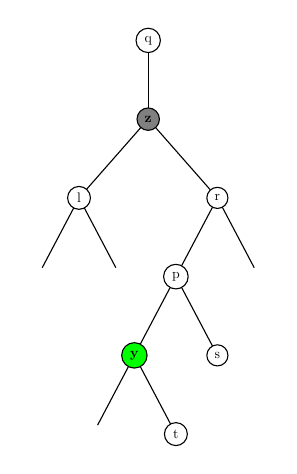
\begin{tikzpicture}[
                    level 2/.style={sibling distance=5em},
                    level 3/.style={sibling distance=3em}
                ]
                    \node {q}
                        child {node[fill=gray]{\textbf{z}}
                            child {node{l}
                                child {node[draw=none] {}}
                                child {node[draw=none] {}}
                            }
                            child {node{r}
                                child {node{p}
                                    child {node[fill=green]{\textbf{y}}
                                        child {node[draw=none] {}}
                                        child {node{t}}
                                    }
                                    child {node{s}}
                                }
                                child {node[draw=none] {}}
                            }
                        };
                \end{tikzpicture}
            }
            

            \column{.1\textwidth}
            \centering
            \uncover<8->{$\longrightarrow$}
        
            \column{.45\textwidth}
            \centering
            \only<8>{%
                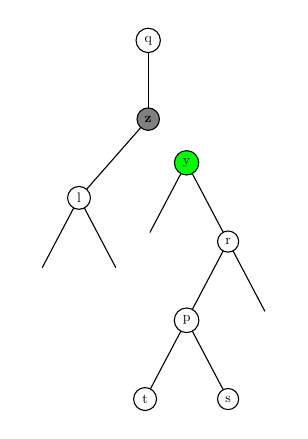
\begin{tikzpicture}[
                    level 2/.style={sibling distance=5em},
                    level 3/.style={sibling distance=3em}
                ]
                    \node {q}
                        child {node[fill=gray]{\textbf{z}}
                            child {node{l}
                                child {node[draw=none] {}}
                                child {node[draw=none] {}}
                            }
                            child {edge from parent[draw=none] node[fill=green]{y}
                                child {node[draw=none] {}}
                                child {node{r}
                                    child {node{p}
                                        child {node{t}}
                                        child {node{s}}
                                    }
                                    child {node[draw=none] {}}
                                }
                            }
                        };
                \end{tikzpicture}
            }

            \only<9->{%
                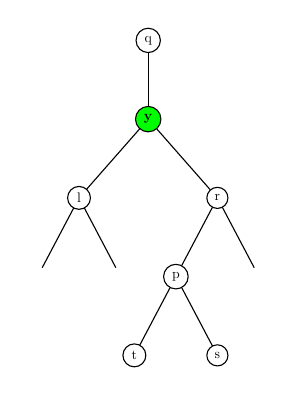
\begin{tikzpicture}[
                    level 2/.style={sibling distance=5em},
                    level 3/.style={sibling distance=3em}
                ]
                    \node {q}
                        child {node[fill=green]{\textbf{y}}
                            child {node{l}
                                child {node[draw=none] {}}
                                child {node[draw=none] {}}
                            }
                            child {node{r}
                                child {node{p}
                                    child {node{t}}
                                    child {node{s}}
                                }
                                child {node[draw=none] {}}
                            }
                        };
                \end{tikzpicture}
            }

        \end{columns}
    \end{columns}
    
\end{frame}


\begin{frame}{Manipulering af BST'er}{Deletion pseudo-kode}
    Vi prøver nu at tage et kig på koden for $\proc{Tree-Delete}(T,z)$.

    \begin{columns}
        \column{.55\textwidth}
        \small
        \begin{itemize}[<+(1)->]
            \item Først, bemærk at vi har en sub-procedure
                $\proc{Transplant}(T,u,v)$, som erstatter knuden $u$ med knuden
                $v$ i træet $T$ 
            \item Linie 1-4 dækker de tilfælde, hvor $z$ kun har et barn, og vi
                bare skal flytte barnet op
            \item Hvis $z$ har to børn finder vi dets successor $y$ i linie 5
            \item Linie 6-9 dækker den case, hvor $y$ ikke er $z$'s højre barn
                \begin{itemize}
                    \item Linie 7 erstatter $y$ med $y$'s højre barn
                    \item Linie 8-9 flytter pointers, så $y$'s højre barn nu er
                        $z$'s højre barn
                \end{itemize}
            \item I Linie 10-12 er $y$ med sikkerhed $z$'s højre barn, og
                vi blot kan erstatte $z$ med $y$ og rykke lidt pointers
            \item Kompleksitet? \uncover<10->{$O(h)$}
        \end{itemize}
    
        \column{.45\textwidth}
        \begin{block}{$\proc{Tree-Delete}(T,z)$}
            \small
        
            \vspace{-\abovedisplayskip}
            \begin{codebox}
                \li \If \alertline<3>$\attrib{z}{left} \isequal \const{NIL}$ 
                    \Then
                \li     \alertline<3>$\proc{Transplant}(T,z,\attrib{z}{right})$
                \li \ElseIf \alertline<3>$\attrib{z}{right} \isequal \const{NIL}$ 
                    \Then
                \li     \alertline<3>$\proc{Transplant}(T,z,\attrib{z}{left})$
                \li \Else 
                        \alertline<4>$y \gets \proc{Tree-Minimum}(\attrib{z}{right})$ 
                \li     \If \alertline<5>$y \neq \attrib{z}{right}$
                        \Then
                \li         \alertline<6>$\proc{Transplant}(T,y,\attrib{y}{right})$
                \li         \alertline<7>$\attrib{y}{right} \gets \attrib{z}{right}$ 
                \li         \alertline<7>$\attrib{\attrib{y}{right}}{p} \gets y$ 
                        \End
                \li     \alertline<8>$\proc{Transplant}(T,z,y)$
                \li     \alertline<8>$\attrib{y}{left} \gets \attrib{z}{left}$
                \li     \alertline<8>$\attrib{\attrib{y}{left}}{p} \gets y$ 
                    \End

            \end{codebox}
        \end{block}
    \end{columns}
\end{frame}


\begin{frame}{Manipulering af BST'er}{Transplant proceduren}
    For god ordens skyld tager vi også lige $\proc{Transplant}$-proceduren.

    \begin{columns}
        \column{.33\textwidth}
        \small
        \begin{block}{$\proc{Transplant}(T,u,v)$}
        
            \vspace{-\abovedisplayskip}
            \begin{codebox}
                \li \If \alertline<2>$\attrib{u}{p} \isequal \const{NIL}$
                    \Then
                \li     \alertline<2>$\attrib{T}{root} \gets v$ 
                \li \ElseIf \alertline<3>$u \isequal \attrib{\attrib{u}{p}}{left}$
                    \Then
                \li     \alertline<3>$\attrib{\attrib{u}{p}}{left} \gets v$
                \li \Else \alertline<3>$\attrib{\attrib{u}{p}}{right} \gets v$
                    \End
                \li \If \alertline<4>$v \neq \const{NIL}$ 
                    \Then
                \li     \alertline<4>$\attrib{v}{p} \gets \attrib{u}{p}$ 
                    \End
            \end{codebox}
        \end{block}
    
        \column{.33\textwidth}
        \small
        \begin{itemize}[<+(1)->]
            \item Linie 1-2 tjekker, om vi skal opdatere $T$'s rod (hvis $u$
                ikke har nogen parent)
            \item Linie 3-5 tjekker, om $u$ er venstre eller højre barn af sin
                parent og indsætter $v$ på rette plads
            \item Linie 6-7 sætter $v$'s parent til at være $u$'s parent, hvis
                ikke $v$ er $\const{NIL}$
        \end{itemize}

        \column{.33\textwidth}
        \centering
        \only<2>{%
            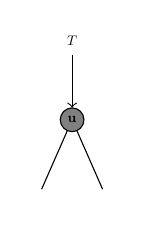
\begin{tikzpicture}
                \node[draw=none] {$T$}
                    child {node[fill=gray] {\textbf{u}} edge from parent[->]
                        child {node[draw=none] {} edge from parent[-]}
                        child {node[draw=none] {} edge from parent[-]}
                    };
            \end{tikzpicture}
        }

        \only<3>{%
            \begin{columns}
                \column{.45\textwidth}
                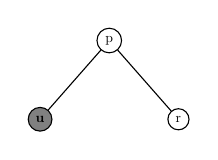
\begin{tikzpicture}
                    \node {p}
                        child {node[fill=gray] {\textbf{u}}}
                        child {node {r}};
                \end{tikzpicture}

                \column{.1\textwidth}
                $\longrightarrow$

                \column{.45\textwidth}
                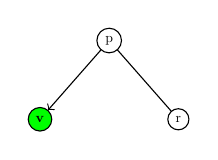
\begin{tikzpicture}
                    \node {p}
                        child {node[fill=green] {\textbf{v}} edge from parent[->]}
                        child {node {r}};
                \end{tikzpicture}

            \end{columns}
            \vfill
            \begin{columns}
                \column{.45\textwidth}
                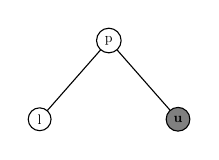
\begin{tikzpicture}
                    \node {p}
                        child {node {l}}
                        child {node[fill=gray] {\textbf{u}}};
                \end{tikzpicture}

                \column{.1\textwidth}
                $\longrightarrow$

                \column{.45\textwidth}
                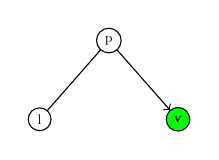
\begin{tikzpicture}
                    \node {p}
                        child {node {l}}
                        child {node[fill=green] {\textbf{v}} edge from parent[->]};
                \end{tikzpicture}

            \end{columns}
        }
        \only<4>{%
            \begin{columns}
                \column{.45\textwidth}
                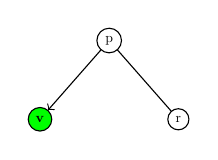
\begin{tikzpicture}
                    \node {p}
                        child {node[fill=green] {\textbf{v}} edge from parent[->]}
                        child {node {r}};
                \end{tikzpicture}

                \column{.1\textwidth}
                $\longrightarrow$

                \column{.45\textwidth}
                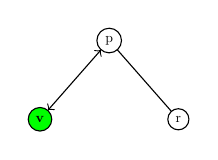
\begin{tikzpicture}
                    \node {p}
                        child {node[fill=green] {\textbf{v}} edge from parent[<->]}
                        child {node {r}};
                \end{tikzpicture}

            \end{columns}
        }
    \end{columns}
\end{frame}


\begin{frame}{Deletion i et BST}{Eksempel}
    \tikzset{level distance=0.8cm}
    \begin{columns}[t]
        \column<1->{.25\textwidth}
        \centering
        $\proc{Tree-Delete}(T,7)$
        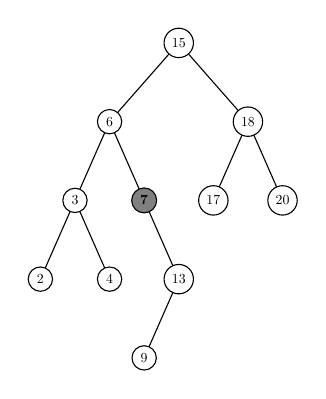
\begin{tikzpicture}
            \node {15}
                child {node {6}
                    child {node {3}
                        child {node {2}}
                        child {node {4}}
                    }
                    child {node[fill=gray] {\textbf{7}}
                        child[missing]{}
                        child {node{13}
                            child {node {9}}
                            child[missing] {}
                        }
                    }
                }
                child {node {18}
                    child {node {17}}
                    child {node {20}}
                };
        \end{tikzpicture}
        
        \column<2->{.25\textwidth}
        \centering
        $\proc{Tree-Delete}(T,6)$
        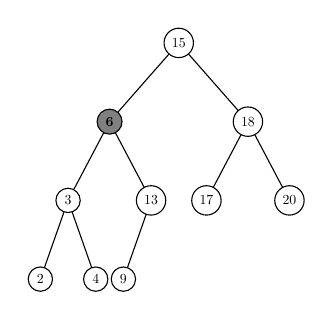
\begin{tikzpicture}[
            level 2/.style={sibling distance=3em},
            level 3/.style={sibling distance=2em},
            ]
            \node {15}
                child {node[fill=gray] {\textbf{6}}
                    child {node {3}
                        child {node {2}}
                        child {node {4}}
                    }
                    child {node{13}
                        child {node {9}}
                        child[missing] {}
                    }
                }
                child {node {18}
                    child {node {17}}
                    child {node {20}}
                };
        \end{tikzpicture}
        
        \column<3->{.25\textwidth}
        \centering
        $\proc{Tree-Delete}(T,15)$
        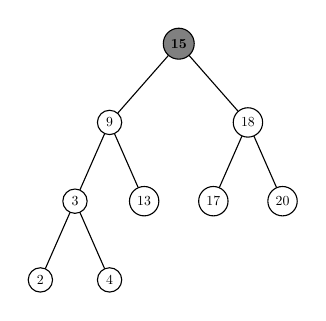
\begin{tikzpicture}
            \node[fill=gray] {\textbf{15}}
                child {node {9}
                    child {node {3}
                        child {node {2}}
                        child {node {4}}
                    }
                    child {node{13}}
                }
                child {node {18}
                    child {node {17}}
                    child {node {20}}
                };
        \end{tikzpicture}
    
        \column<4->{.25\textwidth}
        \centering
        $\proc{Tree-Delete}(T,3)$
        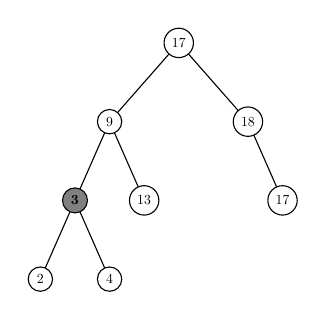
\begin{tikzpicture}
            \node {17}
                child {node {9}
                    child {node[fill=gray] {\textbf{3}}
                        child {node {2}}
                        child {node {4}}
                    }
                    child {node{13}}
                }
                child {node {18}
                    child[missing] {}
                    child {node {17}}
                };
        \end{tikzpicture}
    

    \end{columns}

    \begin{columns}[t]
        \column<5->{.25\textwidth}
        \centering
        $\proc{Tree-Delete}(T,9)$
        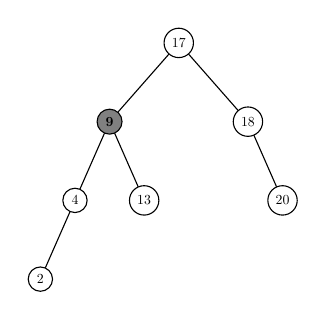
\begin{tikzpicture}
            \node {17}
                child {node[fill=gray] {\textbf{9}}
                    child {node {4}
                        child {node {2}}
                        child[missing] {}
                    }
                    child {node{13}}
                }
                child {node {18}
                    child[missing] {}
                    child {node {20}}
                };
        \end{tikzpicture}
        
        \column<6->{.25\textwidth}
        \centering
        $\proc{Tree-Delete}(T,2)$
        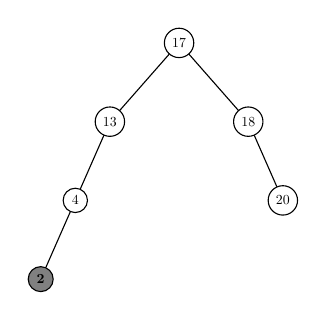
\begin{tikzpicture}
            \node {17}
                child {node {13}
                    child {node {4}
                        child {node[fill=gray] {\textbf{2}}}
                        child[missing] {}
                    }
                    child[missing] {}
                }
                child {node {18}
                    child[missing] {}
                    child {node {20}}
                };
        \end{tikzpicture}
    
        \column<7->{.25\textwidth}
        \centering
        $\proc{Tree-Delete}(T,17)$
        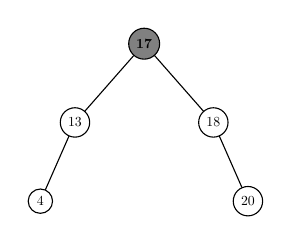
\begin{tikzpicture}
            \node[fill=gray] {\textbf{17}}
                child {node {13}
                    child {node {4}}
                    child[missing] {}
                }
                child {node {18}
                    child[missing] {}
                    child {node {20}}
                };
        \end{tikzpicture}
    
        \column<8->{.25\textwidth}
        \centering
        Finito
        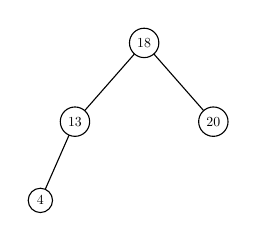
\begin{tikzpicture}
            \node {18}
                child {node {13}
                    child {node {4}}
                    child[missing] {}
                }
                child {node {20}};
        \end{tikzpicture}
    
    \end{columns}
\end{frame}


\begin{frame}{Opsamling}{}
    Vi har brugt hele dagen på at snakke om binære søgetræer.

    \begin{itemize}[<+(1)->]
        \item Det er en smuk datastruktur
        \item De kan bruges som både \alert{dictionaries} (key/value pairs) og
            priority queues
        \item Alle operationer kører i tid proportionelt med højden $h$
            \begin{itemize}
                \item For et balanceret træ med $n$ knuder er højden $\sim \log
                    n$
                \item I værste fald er højden dog ligeså stor som antallet af
                    knuder
            \end{itemize}
        \item Vi har også set, at ChatGPT kan være meget misvisende
    \end{itemize}
\end{frame}


\begin{frame}{Næste gang\ldots}{\ldots er lidt anderledes}
    I næste uge har vi ikke nogen forelæsning. I stedet, så vil der være en
    såkaldt `self-study' session, hvor I får mulighed for at prøve kræfter med
    et eksamenssæt.

    \begin{itemize}
        \item I får 2 timer til at lave et halvt eksamenssæt (den rigtige
            eksamen er 4 timer)
        \item Så bruger vi tiden bagefter på at gennemgå løsningen sammen
        \item I kan enten komme her til lokalet og lave det i en setting, der
            minder om den rigtig eksamenssituation (jeg vil være her, og kan
            hjælpe lidt, selvom det selvfølgelig bryder med
            eksamenssimuleringen)
        \item Eller I kan lave det i jeres gruppe-lokaler, og så bare komme
            herop kl 14.30, hvis I vil være med til at gennemgå løsningen
    \end{itemize}
\end{frame}





\begin{frame}{Tak for i dag!}{Flere exercises..}

    Den bedste måde ikke at snyde sig selv på er lave exercises!

    \begin{figure}[h]
        \centering
        \includegraphics[width=0.8\textwidth]{exercises}
    \end{figure}
    
\end{frame}



\end{document}


